\section{Constructing Converged Projections}

\begin{figure*}
  \centering
  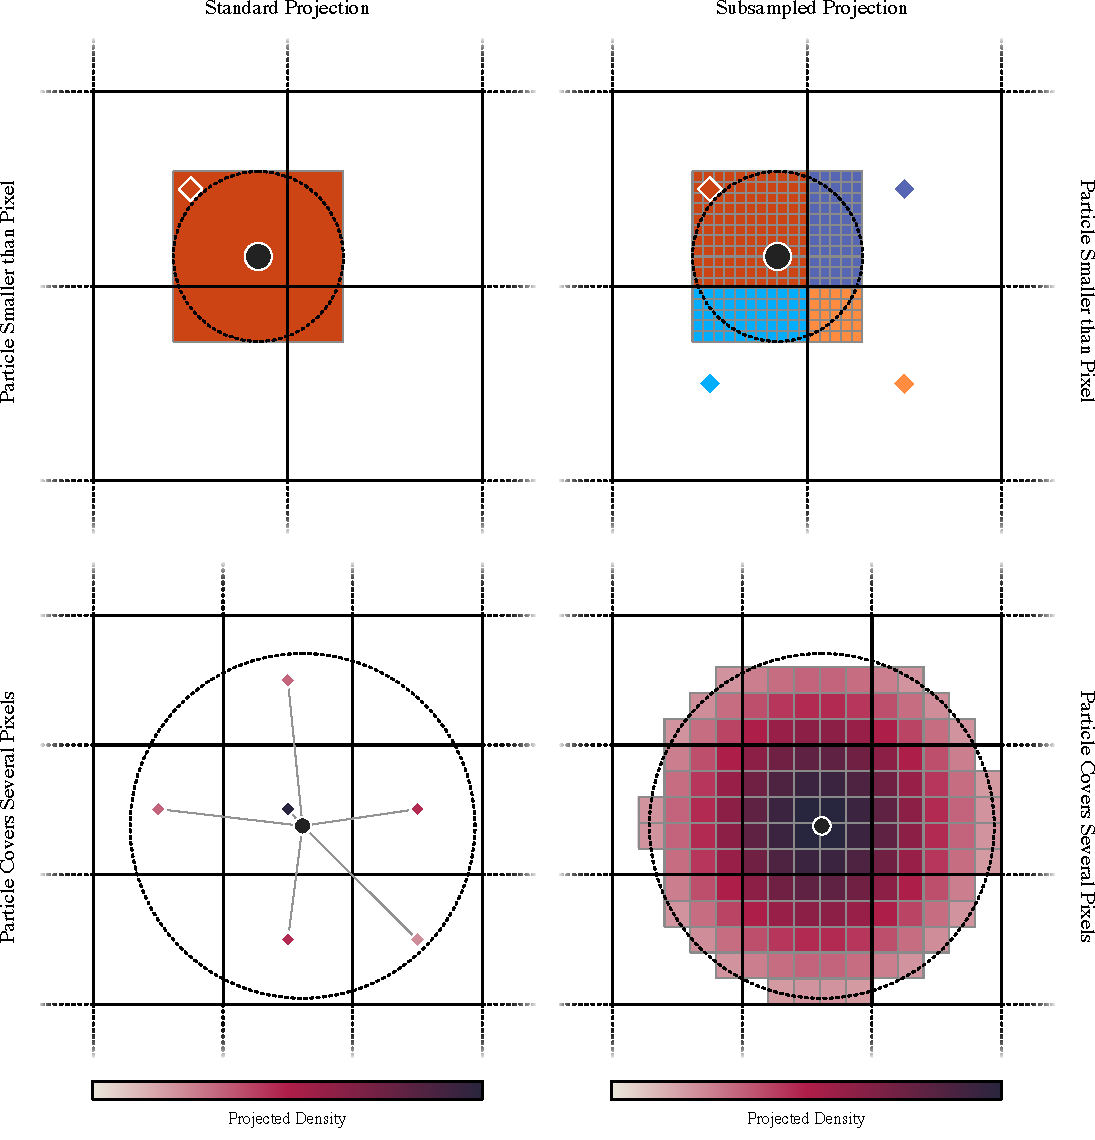
\includegraphics[width=\textwidth]{./plots/algorithm.pdf}
  \caption{Example cases where the size of the smoothing length (kernel extent shown with dashed lines) of a particle (black point) is smaller than a pixel size (top row) and approximately the size of a pixel (bottom row). The columns show the standard projection algorithm (left) and the sub-sampled, new, algorithm (right). The background black grid shows the pixels, with diamonds representing the kernel evaluation points at the centre of relevant pixels. These are omitted in the bottom right image for clarity, and are replaced with a representation of the sub-pixel grid. In the top left panel, the particle is treated as unresolved, and so its entire density contribution is given to the top left pixel, despite the particle overlapping with three other pixels. In the top right, the blitting grid (grey) is used to appropriately apportion the mass over the four pixels (coloured by their contributing sector of the grid). The bottom left panel shows how the particle usually contributes to each pixel using the evaluated value of the kernel at the pixel centre (with each evaluation point coloured by the appropriate projected density). The bottom right shows the subsampled grid, where the kernel is evaluated at each point to ensure a good reconstruction of the kernel gradient.}
  \label{fig:algorithm}
\end{figure*}

In order to construct converged projections of the field, we must re-integrate our ability to assume that the particles are ordered regularly, and that the field is smooth. To do this, we introduce two new measures.

The first, for particles below the field grid size, is termed `blitting'. Here, we construct a pre-calculated high resolution image of the projected kernel (at $N \times N$ pixels, where here $N=32$). If the kernel extent overlaps any pixel boundary, this pre-calculated kernel is overlaid on the pixel grid and each pixel is assigned the kernel contributions that overlap with the pixel.

The second, termed sub-pixel subsampling (or just `subsampling') ensures that each kernel is well resolved by ensuring that at least $N \times N$ sampling points are made available. If the particle overlaps fewer than $N$ pixels in one dimension, sub-pixels are temporarily generated, which are aligned with the pixel boundaries. This ensures that the kernel gradient is well sampled for all particles. It also ensures that for cases where the kernel does not overlap with the pixel centre, but does overlap with some of the pixel area, that contributions are still made.

A demonstration of these two effects, compared to the standard projection scheme, is shown in Fig. \ref{fig:algorithm}. Algorithmically, the `Subsampled' approach looks like:
\begin{enumerate}
  \item Start with a pixel grid full of zeroes.
  \item Pre-calculate an $N \times N$ grid representing the kernel over a smoothing
        length, and store this.
  \item Take all particle positions $\mathbf{r}_{\rm part}$ and particle
        smoothing lengths $h$. For each particle:
  \item Check if $H< 0.25 {\rm d}x$, and if so:
    \begin{enumerate}
      \item Check for overlaps between this particle and
            neighbouring cells. If there are no overlaps, simply add $m/A$ to
            the containing pixel with $A$ the area of the pixel.
      \item If there are overlaps, use the pre-calculated kernel grid to
            spread the appropriate contribution from this particle over the
            relevant neighbouring cells.
    \end{enumerate}
  \item Otherwise:
    \begin{enumerate}
      \item If this is not the case, figure out how many pixels this kernel
            will overlap $n$. If this is smaller than $N$, sub-sample the pixels
            $N/n$ times (rounded up) at positions $\mathbf{r}_{\rm sub}$.
      \item Loop over the sampling points, and evaluate the projected kernel
            $W(|\mathbf{r}_{\rm part} - \mathbf{r}_{\rm sub}|, h) = W_{\rm sub}$.
      \item Find the mean value of $W_{\rm sub}$ for each pixel, and add this
            contribution to each pixel.
    \end{enumerate}
\end{enumerate}

\begin{figure}
  \centering
  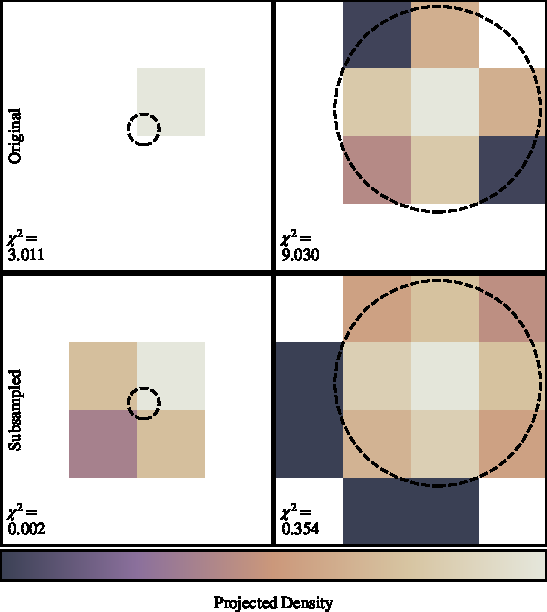
\includegraphics[width=\columnwidth]{./plots/pathalogical/pathalogical_cases.pdf}
  \caption{Two pathological cases (columns) corresponding to the pictorial descriptions in Fig. \ref{fig:algorithm}. Again the kernel extent of the particles is demonstrated using a dashed black line. The two rows show how the standard projection technique (`Original') and the `Subsampled' technique handle a case where the particle is much smaller than the $4\times4$ pixel grid used here (left) and only covers a few pixels (right). $\chi^2$ values are given in the bottom left, relative to a very high resolution downsampled grid (1024$^2$). White pixels show where the kernel was never evaluated; in these pixels the projected density is estimated to be exactly zero.}
  \label{fig:pathalogical}
\end{figure}

In Fig. \ref{fig:pathalogical} we demonstrate how the subsampling technique improves performance on two pathological cases on a $4\times4$ pixel grid. The first, shown in the left column, is where a particle with a small smoothing length overlaps a few neighbouring pixels. In the original scheme, the small smoothing length of the particle means all of its contribution is assigned to one pixel, leading to a large error. The `blitting' grid in the subsampled approach ensures that the contributions to neighbouring pixels are correctly captured.

The right column of Fig. \ref{fig:pathalogical} shows a case where the sub-pixel subsampling increases performance by nearly two orders of magnitude. In the original case, the gradient of the kernel in the outer pixels is poorly sampled, leading to an under-estimation of the projected density in these pixels (and in the case of the top-right pixel, no kernel evaluation at all). The sub-pixel subsampling ensures that the kernel is well sampled and that, even in this challenging case, it is possible to reconstruct an accurate projected density field.

If other particles were present in these images, their contributions would lead to a reduction in the overall error. In the top left panel, neighbouring particles would have their contributions assigned entirely to other pixels, perhaps increasing the accuracy of this method. However, this is a case of one error compensating for another, and in an adaptive environment such consistency in the particle arrangement is never guaranteed.